\documentclass[11pt]{article}
\usepackage{amsmath, amsthm, amssymb, pdfpages} 
\usepackage{fullpage}
\usepackage{hyperref}
\usepackage{graphicx}
\usepackage[capitalize]{cleveref}

% next three for UTF8 to work (for non-ASCII names to work without awkward codes)
\usepackage[T1]{fontenc}
\usepackage{textcomp}
\usepackage[utf8]{inputenc}

% import biblatex with prefered settings
% reuse code and library from LIGERA paper in the same repository
% loads biblatex with all the nice standard options that John determined some time ago!
% this version uses a ``Harvard'' style (first author last name, year in parentheses).
% also loads xpatch

% biblatex
% harvard style
\usepackage[style=authoryear,natbib,maxcitenames=2,doi=false,isbn=false,url=false,backend=bibtex]{biblatex}
% % numeric style
% \usepackage[style=numeric-comp,sorting=none,giveninits=true,doi=false,isbn=false,url=false,backend=bibtex]{biblatex}
% % to have citep etc work without a hitch here...
% \newcommand{\citep}{\cite}
% \newcommand{\citet}{\cite}

% remove "In: " before journal title
\renewbibmacro{in:}{}
% remove language
\AtEveryBibitem{\clearlist{language}}
% remove month
\AtEveryBibitem{\clearfield{month}}
% and also notes
\AtEveryBibitem{\clearfield{note}}
% remove dots between volume and issue
\usepackage{xpatch}
\xpatchbibmacro{volume+number+eid}{%
  \setunit*{\adddot}%
}{%
}{}{}
% put issue in parentheses
\DeclareFieldFormat[article]{number}{\mkbibparens{#1}}

\bibliography{../../manuscripts/zotero, ../../manuscripts/dummy} % biblatex wants this in the preamble...

% path for figures
\graphicspath{ {../data/} }

\usepackage[noT]{kinshipsymbols}
% % copy of \Fst from package `kinshipsymbols`

% some more definitions
\newcommand{\kinMat}{%
  \ensuremath{%
    \mathbf{\Phi}
  }%
  \xspace%
}%
\newcommand{\kinMatStdLim}{%
  \ensuremath{%
    \mathbf{\hat{\Phi}}^\text{std-lim}
  }%
  \xspace%
}%

% for theorems!
\usepackage{amsthm}
%\newtheorem{thm}{Theorem}[section]
\newtheorem*{thm}{Theorem}
%\newtheorem{lem}[thm]{Lemma}
\newtheorem*{lem}{Lemma}
% \newtheorem{lemma}[theorem]{Lemma}

% % double line spacing (PLoS wants this)
% \usepackage{setspace}
% \doublespacing
% spacing smaller than double
\renewcommand{\baselinestretch}{1.2}

\title{\Large \textbf{The effect of population kinship estimation bias in heritability estimation and genetic association}}
\author{Zhuoran Hou$^1$, Alejandro Ochoa$^{1,2,*}$}
\date{}

\begin{document}
\maketitle

\noindent
$^1$ Department of Biostatistics and Bioinformatics, Duke University, Durham, NC 27705, USA \\
$^2$ Duke Center for Statistical Genetics and Genomics, Duke University, Durham, NC 27705, USA \\
$^*$ Corresponding author: \texttt{alejandro.ochoa@duke.edu}


\begin{abstract}
  Population kinship matrices are estimated for a variety of applications, including estimation of heritability and to control for population structure in genetic association studies.
  Recent work found that the most common family of kinship estimators can be severely biased.
  In this work, we investigate the effect of this kinship bias on the two downstream applications of heritability estimation and genetic association.
  We present a novel trait simulation strategy that accurately parametrizes heritability, even when utilizing real genotypes.
  Using these simulations, we find that heritability estimation becomes biased when using such biased kinship matrices.
  Remarkably however, this kinship bias does not affect genetic associations based on either Principal Components Analysis (PCA) or Linear Mixed-effects Models (LMM).
  Lastly, we explain our empirical observations using theory.
  In particular, the exact form of the bias of the standard kinship estimator is such that it is compensated for by fitting the intercept in both PCA and LMM approaches, which model population structure via covariates, suggesting that only downstream applications with this precise arrangement will be robust to this kinship bias.
\end{abstract}

% \clearpage

% \tableofcontents

\clearpage
	
\section{Introduction}

% direct copy from Part II
Kinship is utilized in principal components analyses and linear-mixed effects models to correct for structure in Genome-Wide Association Studies (GWAS) \citep{xie_combining_1998,yu_unified_2006, aulchenko_genomewide_2007, price_principal_2006, astle_population_2009,kang_efficient_2008, kang_variance_2010, zhou_genome-wide_2012, loh_efficient_2015, sul_population_2018} and to estimate genome-wide heritability \citep{yang_common_2010, yang_gcta:_2011, speed_improved_2012}.
The most commonly-used kinship estimator \citep{price_principal_2006, astle_population_2009, rakovski_kinship-based_2009, thornton_roadtrips:_2010, yang_common_2010, yang_gcta:_2011, zhou_genome-wide_2012, speed_improved_2012, speed_relatedness_2015, loh_efficient_2015, wang_efficient_2017, sul_population_2018} was recently determined to have a complex bias \citep{ochoa_fst2, weir_unified_2017}.

Heritability has long been estimated from the trait correlation between close relatives, particularly identical and fraternal twins, or siblings \citep{falconer_introduction_1996}.
These initial estimation approaches were based on a regression model \citep{falconer_introduction_1996}.
A different model was needed to achieve accurate estimates when estimating on more distant relatives, such as the variance component model of the SOLAR approach \citep{almasy_multipoint_1998}, which is based on estimating kinship from pedigrees.
This idea was extended from pedigrees to populations with the GCTA approach \citep{yang_common_2010, yang_gcta:_2011}, which has spawned much research \citep{visscher_commentary_2010, speed_improved_2012, krishna_kumar_limitations_2016, yang_gcta-greml_2016, jiang_high-dimensional_2016}.
However, we previously found that the most common family of kinship estimators employed by these approaches for populations can be severely biased \citep{ochoa_fst2}.
\citet{speed_improved_2012} focused on some biases related to other assumptions of the multivariate normal heritability model, but biases in kinship estimation were not known or included in these evaluations.

There are alternative approaches for estimating heritability, such as LD Score Regression \citep{bulik-sullivan_ld_2015} and SumHer \citep{speed_sumher_2019}, which we do not consider in this proposal since they are not based on kinship matrices.


\section{Methods}

\subsection{Genetic model}

Suppose there are $m$ biallelic loci and $n$ diploid individuals.
The genotype $\xij \in \{0,1,2\}$ at a locus $i$ of individual $j$ is encoded as the number of reference alleles, for a preselected but otherwise arbitrary reference allele per locus.
These genotypes can be treated as random variables structured according to relatedness.
If \kt is the kinship coefficient of two individuals $j$ and $k$, and \pit is the ancestral allele frequency at locus $i$, then under the kinship model \citep{ochoa_fst1,ochoa_fst2} the expectation and covariance are given by
\begin{align*}
  \E[\mathbf{X}]
  =
    2 \mathbf{p} \mathbf{1}_n^\intercal
  ,
  \quad\quad
  \Cov(\mathbf{x}_i)
  =
    4 \pit (1-\pit) \kinMat
    ,
\end{align*}
where $\mathbf{x}_i$ is the length-$n$ column vector of genotypes at locus $i$, $\mathbf{X} = (\mathbf{x}_i^\intercal)$ is the complete $m \times n$ genotype matrix, $\kinMat = (\kt)$ is the $n \times n$ kinship matrix, $\mathbf{p} = (\pit)$ is a length-$m$ column vector of ancestral allele frequencies, $\mathbf{1}_n = (1)$ is a length-$n$ column vector where every element is 1, and the $\intercal$ superscript denotes matrix transposition.
Both kinship ($\kinMat$) and ancestral allele frequencies ($\mathbf{p}$) are parameters that depend on the choice of ancestral population, for which the Most Recent Common Ancestor (MRCA) population is the most sensible choice \citep{ochoa_fst1,ochoa_fst2}.
In this work, to simplify notation, we omit cumbersome notation that marks this dependence of parameters on the choice of ancestral population, not do we explicitly condition on the ancestral population when calculating expectations and covariances as done in previous work, although it is done implicitly.
This and later notation is summarized in \cref{tab:notation}.

\begin{table}[b!]
  \centering
  \caption{\textbf{Mathematical notation.}}
  \label{tab:notation}
  \begin{tabular}{lll}
    \hline
    Variable                     & Dimensions   & Description                  \\
    \hline
    $m$                          & $1$          & Number of loci               \\
    $n$                          & $1$          & Number of individuals        \\
    $i$                          & $1$          & Locus (variant) index        \\
    $j,k$                        & $1$          & Individual indexes           \\
    $\mu$                        & $1$          & Trait mean                   \\
    $\sigma^2$                   & $1$          & Trait variance scale         \\
    $h^2$                        & $1$          & (Narrow-sense) Heritability  \\
    $\mathbf{X} = (\xij)$        & $m \times n$ & Genotype matrix              \\
    $\mathbf{x}_i = (\xij)$      & $n \times 1$ & Genotype vector at locus $i$ \\
    $\mathbf{y}$                 & $n \times 1$ & Trait vetor                  \\
    $\alpha$                     & $1$          & Intercept                    \\
    $\mathbf{\beta} = (\beta_i)$ & $m \times 1$ & Effect size coefficients     \\
    $\mathbf{\epsilon}$          & $n \times 1$ & Non-genetic random effect    \\
    $\mathbf{p} = (\pit)$        & $m \times 1$ & Ancestral allele frequencies \\
    $\kinMat = (\kt)$      & $n \times n$ & Kinship matrix               \\
    $\mathbf{1}_n$               & $n \times 1$ & Vector of ones               \\
    $\mathbf{I}_n$               & $n \times n$ & Identity matrix              \\
    \hline
  \end{tabular}
\end{table}

The length-$n$ quantitative trait vector $\mathbf{y}$ for all individuals is assumed to follow a linear polygenic model,
\begin{equation}
  \label{eq:trait}
  \mathbf{y}
  =
  \mathbf{1}_n \alpha + \mathbf{X}^\intercal \mathbf{\beta}  + \mathbf{\epsilon},
\end{equation}
where $\alpha$ is the intercept coefficient, $\mathbf{\beta} = (\beta_i)$ is a length-$m$ column vector of effect size coefficients for each locus $i$ (which may be zero), and $\mathbf{\epsilon}$ is a length-$n$ column vector of non-genetic effects.
To analyze the covariance structure of the trait, we shall treat $\alpha$ and $\mathbf{\beta}$ are fixed parameters, while $\mathbf{X}$ and $\mathbf{\epsilon}$ are random.
The non-genetic effects are assumed to be independent with variance $(1-h^2) \sigma^2$ given by the total trait variance scale $\sigma^2$ and the narrow-sense heritability $h^2$:
\begin{align*}
  \E[\mathbf{\epsilon}]
  =
  \mathbf{0}_n
  ,
  \quad\quad
  \Cov(\mathbf{\epsilon})
  =
  (1-h^2) \sigma^2 \mathbf{I}_n
  ,
\end{align*}
where $\mathbf{0}_n$ is a length-$n$ column vector of zeroes.
The expectation of the trait is therefore
\begin{align*}
  \E[\mathbf{y}]
  = \alpha \mathbf{1}_n + \E \left[ \mathbf{X}^\intercal \right] \mathbf{\beta} + \E[\mathbf{\epsilon}]
%  = \alpha \mathbf{1}_n + 2 \mathbf{1}_n \mathbf{p}^\intercal \mathbf{\beta}
  = \mu \mathbf{1}_n
  , \quad\quad \text{where} \quad\quad
  \mu 
  =
  \alpha + 2 \mathbf{p}^\intercal \mathbf{\beta}
  .
\end{align*}
The covariance matrix of the trait is
\begin{align*}
  \Cov(\mathbf{y})
  =
  \left( \sum_{i=1}^m \Cov(\mathbf{x}_i) \beta_i^2 \right) + \Cov(\mathbf{\epsilon})
  =
  \kinMat \left( \sum_{i=1}^m 4 \pit (1-\pit) \beta_i^2 \right) + (1-h^2) \sigma^2 \mathbf{I}_n
  .
\end{align*}
Therefore, we can write the covariance in terms of the heritability and the overall variance scale, in a formulation that matches previous work \citep{yang_common_2010, yang_gcta:_2011, speed_improved_2012}:
\begin{equation*}
  \Cov(\mathbf{y})
  =
  \sigma^2 \left( h^2 2 \kinMat  + (1-h^2) \mathbf{I}_n \right)
  , \quad\quad \text{where} \quad\quad
  \sigma^2 h^2 
  = 
  \sum_{i=1}^m 2 \pit (1-\pit) \beta_i^2
  .
\end{equation*}
This last equation suggests a clear definition for the single-locus $i$ contribution to the heritability, given by
\begin{equation}
  \label{eq:herit_per_locus}
  h^2_i
  =
  2 \pit (1-\pit) \beta_i^2 \sigma^{-2},
\end{equation}
which is such that the total heritability is a sum of these single-locus heritabilities: $h^2 = \sum_{i=1}^m h^2_i$.
Since the earlier expectations and covariances are conditioned on the choice of ancestral population, and given in terms of parameters that depend on it (\pit and $\kinMat$), then the parameters $\mu, \sigma^2, h^2$ are all also dependent on the choice of ancestral population.

The parametrization of our model is equivalent to setting separate absolute scales to the genetic and environment variance components, as $\sigma^2_G = h^2 \sigma^2$ and $\sigma^2_E = (1-h^2) \sigma^2$, respectively, which results in $\sigma^2_G + \sigma^2_E = \sigma^2$ and $\sigma^2_G / (\sigma^2_G + \sigma^2_E) = h^2$, as desired.

The factor of two in front of $\kinMat$ is traditionally there so that for an unstructured population
$2 \kinMat = \mathbf{I}_n$, in which case the trait covariance simplifies to
$\Cov(\mathbf{y}) = \sigma^2 \mathbf{I}_n$ for any value of $h^2$.
More broadly, the variance of the trait for any outbred individual is $\sigma^2$ under this parametrization.
In many previous presentations this factor of 2 does not appear there explicitly, but instead the kinship matrix is defined as $2 \kinMat$ \citep{yang_gcta:_2011, speed_improved_2012}.

\subsection{Multivariate Normal estimation model}

Here we focus on heritability estimation from the Multivariate Normal (MVN) variance component model, namely \citep{speed_improved_2012, yang_gcta:_2011}
\begin{equation}
  \label{eq:heritMVN}
  \mathbf{y}
  \sim
  \text{MVN}
  \left(
    \mu \mathbf{1},
    \sigma^2 \left(
      2 h^2 \kinMat
      + (1-h^2) \mathbf{I}_n
      \right)
  \right)
  .
\end{equation}
Note that, by construction, the above trait vector has the same mean and covariance matrix of the genetic trait model in \cref{eq:trait}.
However, the trait in \cref{eq:heritMVN} is not drawn from genotypes anymore, but solely from the kinship matrix; for this reason we refer to this as a \textit{MVN} trait, in contrast to the \textit{genetic} trait model in \cref{eq:trait}.

This MVN trait model (from \cref{eq:heritMVN}) is justified as arising from the genetic trait model (from \cref{eq:trait}) in the limiting case of infinite causal locus effects, each with equal per-locus variance (heritability) according to \cref{eq:herit_per_locus} (equal $\pit (1-\pit) \beta_i^2$ for all $i$), the condition under which the genetic trait approaches the MVN distribution as a consequence of the multivariate central limit theorem.
However, convergence may be slower in practice since both effect sizes ($\beta_i$) and ancestral allele frequencies (\pit) vary for realistic causal loci, so the product $\pit (1-\pit) \beta_i^2$ is not expected to be the same at all causal loci $i$.
Another way of stating the difference is that \cref{eq:trait} and \cref{eq:heritMVN} agree in the first two moments, but disagree in higher moments.

\subsection{Kinship estimation}

\subsubsection{Standard kinship estimator}

The ``standard'' kinship estimator is the most common estimator employed across various applications for population structure \citep{astle_population_2009, speed_relatedness_2015, wang_efficient_2017}, including
heritability estimation \citep{speed_improved_2012, speed_relatedness_2015, speed_reevaluation_2017}
and genetic association tests based on PCA \citep{price_principal_2006},
LMMs \citep{astle_population_2009, zhou_genome-wide_2012, loh_efficient_2015, sul_population_2018}
and other models \citep{rakovski_kinship-based_2009, thornton_roadtrips:_2010}.
The popular heritability estimation approach GCTA \citep{yang_common_2010, yang_gcta:_2011} employs a variant of this estimator detailed in the next paragraph.
The standard estimator, and its almost sure limit as the number of loci $m$ and number of individuals $n$ go to infinity \citep{ochoa_fst2}, are given by
\begin{align}
  \label{eq:kinship_std}
  \ktHatStd
  &=
    \frac{1}{m} \sum\limits_{i=1}^m \frac{\left( \xij - 2 \pith \right) \left( \xij[k] - 2 \pith \right)}{4 \pith \left( 1-\pith \right)}
  \\
  \label{eq:kinship_std_lim}
  &\toasNM
    \frac{\kt -\bar{\varphi}_j -\bar{\varphi}_k + \bar{\varphi}}{1 - \bar{\varphi}}
    ,
\end{align}
where \ktHatStd is the estimated kinship of individuals $j$ and $k$,
$\pith = \frac{1}{2n} \sum_{j=1}^n \xij$ is the standard ancestral allele frequency estimator,
$\bar{\varphi}_j = \frac{1}{n} \sum_{k=1}^n \kt$ is the mean kinship of individual $j$ with all others, and
$\bar{\varphi} = \frac{1}{n^2} \sum_{j=1}^n \sum_{k=1}^n \kt$ is the overall mean kinship.
This is a complex bias that varies for every pair of individuals, and which is on average a downward bias.
(Note that the mean estimate, or $\frac{1}{n^2} \sum_{j=1}^n \sum_{k=1}^n \ktHatStd$, is algebraically zero, regardless of the true value of the mean kinship.)

Variants of this approach that weigh loci according to linkage disequilibrium \citep{speed_reevaluation_2017, wang_efficient_2017} do not alter the bias calculated above, since the same bias is present in each individual locus \citep{ochoa_fst2}.
Our previous work also considered a more general form where the ancestral allele frequency estimator $\pith = \frac{1}{2} \sum_{j=1}^n w_j \xij$ is calculated with weights $w_j$ per individual $j$ (such that $\sum_{j=1}^n w_j = 1$), and found that these weights alter the values of the bias terms $\bar{\varphi}_j$ and $\bar{\varphi}$ to be weighted averages, but no choice of weights eliminates these biases \citep{ochoa_fst2}.
Such weighted \pith estimates encompass the best unbiased linear estimator \citep{astle_population_2009, thornton_roadtrips:_2010}, with weights corresponding to
$
\mathbf{w} = ( \mathbf{1}^\intercal \kinMat^{-1} \mathbf{1} )^{-1} \mathbf{1}^\intercal \kinMat^{-1}.
$

\subsubsection{GCTA kinship estimator}

The GCTA software \citep{yang_gcta:_2011} estimate what they refer to as a Genetic Relatedness Matrix (GRM), which is evidently twice a kinship matrix estimate due to the similarity to \cref{eq:kinship_std} and due to the historical connection between kinship and heritability in \cref{eq:heritMVN} and in previous work \citep{falconer_introduction_1996}.
In fact, the GCTA kinship estimates for two different individuals is identical to \cref{eq:kinship_std} (after taking into account the factor of 2 in \cref{eq:heritMVN}):
$$
\ktHatNamed{GCTA} = \ktHatStd \quad\quad \text{for} \quad\quad j \ne k.
$$
The GCTA kinship estimator differs from the standard estimator only for $j=k$ \citep{yang_gcta:_2011}, where the estimator and its limit are instead given by \citep{ochoa_fst2}:
% % copy from Part II:
% The limits of the ratio-of-means versions of two more \ft estimators \citep{yang_gcta:_2011} are
% \begin{equation}
%   \label{eq:fHatsGcta}
%   \begin{split}
%     \ftHatStdII
%     &= 1 - \frac{\sum\limits_{i=1}^m \xij(2-\xij)}{2 \sum\limits_{i=1}^m \pith \left( 1-\pith \right)}
%     \toas \frac{\ft - \bar{\varphi}^T}{1 - \bar{\varphi}^T} , \\
%     %%     
%     \ftHatStdIII
%     &= \frac{\sum\limits_{i=1}^m \xij^2 - \left( 1 + 2\pith \right) \xij + 2\left(\pith \right)^2}{2 \sum\limits_{i=1}^m \pith \left( 1-\pith \right)}
%     \toas \frac{ \ft + \bar{\varphi}^T - 2 \bar{\varphi}_j^T }{1 - \bar{\varphi}^T}.
%   \end{split}
% \end{equation}
% GCTA uses version III.
% \begin{equation}
%   \label{eq:kjjHatGctaROM}
%   \begin{split}
%     \ktHatNamed{GCTA}
%     &= \frac{1}{2} + \frac{\sum\limits_{i=1}^m \xij^2 - \left( 1 + 2\pith \right) \xij + 2\left(\pith \right)^2}{4 \sum\limits_{i=1}^m \pith \left( 1-\pith \right)}
%     \toas
%     \frac{ \kt - \bar{\varphi}_j^T }{1 - \bar{\varphi}^T}.
%   \end{split}
% \end{equation}
% This is the real MOR version, removed $T$s:
\begin{align}
  \label{eq:kinship_gcta_self}
  \ktHatNamed[j]{GCTA}
  &=
    \frac{1}{2} + \frac{1}{m} \sum_{i=1}^m \frac{\xij^2 - \left( 1 + 2\pith \right) \xij + 2 \pith^2}{4 \pith \left( 1-\pith \right)}
  \\
  \label{eq:kinship_gcta_self_lim}
  &\toasNM
    \frac{ \kt[j] - \bar{\varphi}_j }{1 - \bar{\varphi}}
    .
\end{align}

\subsubsection{Popkin kinship estimator}

The popkin (population kinship) estimator is given by \citep{ochoa_fst2}
\begin{equation}
  \label{eq:popkin}
  \begin{split}
    \Ajk
    &=
    \frac{1}{m} \sum_{i=1}^m (\xij-1)(\xij[k]-1) - 1
    , \\
    \AMinHat
    &=
    \min_{u \ne v} \frac{1}{|S_u||S_v|} \sum_{j \in S_u} \sum_{k \in S_v} \Ajk
    , \\
    \ktHatNew
    &= 1 - \frac{\Ajk}{\AMinHat},
  \end{split}
\end{equation}
where $S_u$ are subpopulations that partition individuals.
This estimator is accurate ($\ktHatNew \toas \kt$) under the assumption that \AMinHat is calculated over individual pairs whose true kinship is zero.
In other words, the two subpopulations $S_u$ and $S_v$ with the minimum mean \Ajk value should have its true mean kinship value \kt be zero.

\subsection{Heritability and genetic association software}

TODO: state versions, download links, etc.

Outline:
\begin{itemize}
\item SOLAR-Eclipse (herit only) \citep{almasy_multipoint_1998}.
\item GCTA (both heritability and genetic association) \citep{yang_gcta:_2011}.
\item PCA: used plink2 (genetic association only) \citep{chang_second-generation_2015}.
\end{itemize}

\subsection{Simulations}

\subsubsection{Trait simulation algorithm}

Suppose the genotype matrix $\mathbf{X}$ is available, and we have fixed values for the number of causal loci $m_1$, the trait mean, variance scale, and heritability ($\mu, \sigma^2, h^2$).
The goal is to choose the intercept $\alpha$ and draw random effect sizes $\mathbf{\beta}$ that result in the desired trait parameters.
First we randomly select $m_1$ loci to be causal, and subset the genotype matrix $\mathbf{X}$ and ancestral allele frequency vector $\mathbf{p}$ so that from this point on they contain only those causal loci (they now have dimensions $m_1 \times n$ and length $m_1$, respectively).

Below we divide the algorithm into two steps: (1) scaling the effect sizes, and (2) centering the trait.
Each step forks into two cases: whether the true ancestral allele frequencies $\mathbf{p}$ are known or not (the latter requires a known kinship matrix $\kinMat$).

\textbf{Scaling effect sizes.}
The initial effect sizes $\beta_i$ are drawn independently from a standard normal distribution:
$$
\beta_i \sim \text{N}(0, 1).
$$

First we consider the simpler case of known ancestral allele frequencies $\mathbf{p} = (\pit)$.
The initial genetic variance scale is
$$
\sigma^2_0
=
\sum_{i=1}^{m_1} 2 \pit (1-\pit) \beta_i^2
.
$$
We obtain the desired variance by dividing each $\beta_i$ by $\sigma_0$ (which results in a variance of 1) and then multiply by $h \sigma$ (which results in the desired variance of $h^2 \sigma^2$).
Combining both steps, the update is
$$
\mathbf{\beta}
\leftarrow
\mathbf{\beta} \frac{ h \sigma }{\sigma_0}
.
$$

Now we consider the case of unknown ancestral allele frequencies but known kinship matrix.
First, sample estimates $\mathbf{\hat{p}} = (\pith)$ of the ancestral allele frequencies are constructed from the genotype data as
$$
\pith
=
\frac{1}{2n} \mathbf{1}_n^\intercal \mathbf{x}_i
.
$$
Although this estimator is unbiased ($\E[\mathbf{\hat{p}}] = \mathbf{p}$), the resulting variance estimates of interest $\pith \left( 1-\pith \right)$ are downwardly biased \citep{ochoa_fst2}:
$$
\E \left[ \pith \left( 1-\pith \right) \right]
=
\pit(1-\pit) (1 - \bar{\varphi})
,
$$
where $\bar{\varphi} = \frac{1}{n^2} \mathbf{1}_n^\intercal \kinMat \mathbf{1}_n$ is the mean kinship coefficient in the data.
Therefore the initial genetic variance scale, estimated as
$$
\hat{\sigma}^2_0
=
\sum_{i=1}^{m_1} 2 \pith (1-\pith) \beta_i^2
,
$$
has an expectation of
$$
\E \left[ \hat{\sigma}^2_0 \right]
=
\sigma^2_0 (1 - \bar{\varphi})
.
$$
Therefore, assuming that this additional factor $(1 - \bar{\varphi})$ is known, the update
$$
\mathbf{\beta}
\leftarrow
\mathbf{\beta} \frac{ h \sigma \sqrt{1-\bar{\varphi}} }{\hat{\sigma}_0}
$$
results in the desired variance.

\textbf{Centering the trait.}
Here we consider the problem of selecting the intercept coefficient $\alpha$ that, together with the previous effect size coefficient vector $\mathbf{\beta}$, result in the desired trait mean $\mu$.

When ancestral allele frequencies are known, the trait can be centered precisely.
Given our model, we obtain the desired overall trait mean $\mu$ by choosing the intercept coefficient to be
$$
\alpha 
=
\mu - 2 \mathbf{p}^\intercal \mathbf{\beta}
.
$$

When ancestral allele frequencies are unknown, the solution is to choose the intercept coefficient
\begin{align*}
  \alpha 
  =
  \mu - 2 \hat{\bar{p}} \mathbf{1}_{m_1}^\intercal \mathbf{\beta}
  , \quad\quad
  \hat{\bar{p}}
  =
  \frac{1}{m_1} \mathbf{1}_{m_1}^\intercal \mathbf{\hat{p}}
  =
  \frac{1}{ 2 m_1 n } \mathbf{1}_{m_1}^\intercal \mathbf{X}^\intercal \mathbf{1}_n
  =
  \frac{1}{2} \bar{X}
  ,
\end{align*}
where $\mathbf{1}_{m_1}$ is a length-$m_1$ column vector of ones.
Note that this overal mean allele frequency $\hat{\bar{p}}$ is computed among causal loci only.
This works very well in practice since $\mathbf{\beta}$ is drawn randomly, so it is uncorrelated to $\mathbf{p}$ and therefore
$$
\frac{1}{m_1} \mathbf{p}^\intercal \mathbf{\beta}
=
\frac{1}{m_1} \sum_{i=1}^{m_1} \pit \beta_i
\approx
\left( \frac{1}{m_1} \sum_{i=1}^{m_1} \pit \right)
\left( \frac{1}{m_1} \sum_{i=1}^{m_1} \beta_i \right)
=
\frac{1}{m_1}
\bar{p}
\mathbf{1}_{m_1}^\intercal \mathbf{\beta}
$$
is a good approximation.

Now we discuss why the more obvious naive approach, which would be to center the trait using estimated ancestral allele frequencies as
$
\alpha 
=
\mu - 2 \mathbf{\hat{p}}^\intercal \mathbf{\beta}
,
$
does not work.
This approach is equivalent to centering genotypes at each locus as
$$
\mathbf{y} = \alpha \mathbf{1}_n + \sum_{i=1}^{m_1} (\mathbf{x}_i - 2 \pith \mathbf{1}_n) \beta_i + \mathbf{\epsilon}.
$$
However, this operation introduces a distortion in the covariance of the genotypes \citep{ochoa_fst2}: 
$$
\Cov \left( \mathbf{x}_i - 2 \pith \mathbf{1}_n \right)
=
\pit ( 1 - \pit ) \left( 
\kinMat 
+ \bar{\varphi} \mathbf{1}_n \mathbf{1}_n^\intercal 
- \mathbf{\varphi} \mathbf{1}_n^\intercal 
- \mathbf{1}_n \mathbf{\varphi}^\intercal 
\right),
$$
where $\bar{\varphi}$ is the overall mean kinship, as before, and $\mathbf{\varphi} = \frac{1}{n} \kinMat \mathbf{1}_n$ is a length-$n$ column vector of per-row mean kinship values.
These undesireable distortions propagate to the trait, which we confirmed in simulations (not shown).
%It is not clear how to correct these distortions after centering the trait as shown above.
Note that the intercept version we chose instead does not induce this genotype centering, which prevents the undesireable distortions in the trait covariance.

\subsubsection{Admixture simulation for genotype matrices}

TODO: describe the BNPSD simulation.

\section{Results}

\subsection{Empirical demonstration of biases in heritability estimation}

Here we consider the effect of kinship estimator bias in heritability estimation.
We use simulated genotypes and traits, and either estimate kinship matrices from these genotypes or we show the effect of asymptotic estimator bias based on previously-calculated limits.
In particular, we consider the true kinship matrix of the simulation,
the unbiased popkin estimator in \cref{eq:popkin},
the standard kinship estimator in \cref{eq:kinship_std}
and its limit in \cref{eq:kinship_std_lim},
and the GCTA estimator in \cref{eq:kinship_gcta_self} and its limit in \cref{eq:kinship_gcta_self_lim}.
Lastly, we also consider two simulated trait types, namely the genetic trait in \cref{eq:trait} and the MVN trait (or infinitesimal approximation) in \cref{eq:heritMVN}.
Each scenario was replicated 10 times, in each case producing a new genotype matrix as well as a new genetic and MVN traits.

First we considered a setting where there is only population structure (absence of family structure).
We find that all estimates based on the genetic trait are upwardly biased, including that based on the true kinship matrix of the simulation (\cref{fig:herit_estimation_g1}).
In this case (genetic trait) the GCTA kinship estimates result in heritability estimates without an apparent bias, though its variance is very high.
For the MVN trait case, the true kinship matrix results in unbiased estimation, as expected since here the model is fully specified correctly (the MVN trait assumption holds, and the true kinship matrix is used).
The rest of the estimators and limits are biased for MVN traits too, although the direction varies for different cases:
all kinship estimates underestimate heritability, while the GCTA limit overestimates it.
Many of the overestimates across kinship variants and trait simulation types result in values near or at one.

\begin{figure}[bp!]
  \centering
  \includegraphics[width=6in]{../data/{herit-estimates-n5000-m100000-k3-f0.3-s0.5-mc100-h0.8-g1-r10}.pdf}
  \caption{
    {\bf Heritability estimation by GCTA with various kinship matrices and trait simulation types, admixture structure only.}
    Oracle kinship matrices rely on the true kinship matrix being known (unknown in practice), while estimated kinship matrices are obtained from observed genotypes and are what is used in practice.
    Genetic traits are simulated from genotypes, whereas MVN traits are simulated from the Multivariate Normal model, which is itself used to infer heritability but is unrealistic since it does not depend on any genotypes.
    Genotypes and traits were simulated for $n = 5000$ individuals, $m = 100000$ loci, for 10 replicates, from an admixture simulation ($K = 3$ ancestral subpopulations, $\Fst = 0.3$ for admixed individuals, bias coefficient of $s = 0.5$), no family structure, and the traits had a true heritability of $h^2 = 0.8$ and $m_1 = 100$ causal loci).
  }
  \label{fig:herit_estimation_g1}
\end{figure}

Since traditional heritability estimation is based on family structure, we decided to consider a simulation including both population and family structure.
Simply adding siblings results in striking changes in estimation biases (\cref{fig:herit_estimation_g2}).
Most versions of this analysis yield estimates with lower variance and bias when siblings are included, and the proportion of estimates close to 1 is sharply reduced.
Another large differences is for the GCTA kinship limit, which is near one in the absence of siblings, and are instead downwardly biased when siblings are present.
We still observe that all estimates on the genetic trait are upwardly biased.
Moreover, although the GCTA estimated kinship appeared to ahve low bias in the absence of siblings, the inclusion of siblings reduces their variance and reveals an updard bias in these estimates too.
For the MVN trait, now all estimates are downwardly biased, except for the true kinship matrix (which is expected to be unbiased), and possibly the limit of the standard kinship estimator.

\begin{figure}[bp!]
  \centering
  \includegraphics[width=6in]{../data/{herit-estimates-n5000-m100000-k3-f0.3-s0.5-mc100-h0.8-g2-r10}.pdf}
  \caption{
    {\bf Heritability estimation by GCTA with various kinship matrices and trait simulation types, admixture plus family structure (siblings).}
    Like \cref{fig:herit_estimation_g1}, but proximal individuals (with the most similar ancestries) were mated to simulate siblings, and only the second generation (the siblings) were used to estimate heritability.
  }
  \label{fig:herit_estimation_g2}
\end{figure}

In all these cases (\cref{fig:herit_estimation_g1,fig:herit_estimation_g2}) we find that kinship estimates do not result in the same estimates, on average, as their limits (expected as the number of loci goes to infinity).
In all but one of these cases, heritability estimates are downwardly biased when estimated kinship matrices are used compared to the limits of their respective kinship estimators.
This suggests that kinship estimation variance results in an additional downward bias in heritability estimation, compared to the bias due to kinship estimator bias.
We also find that estimation from proper, genetic traits, is biased under the MVN model on which GCTA's inference is based.
Although MVN traits result in unbiased estimation under the true kinship matrix, this is an impractical scenario since the true kinship matrix is never known and true traits are never MVN.

Overall, since true traits are more like our genetic trait simulation, we expect there to be a heritability upward bias due to performing inference with the misspecified MVN model, and a separate downward bias due to the noise in kinship estimation.
These biases must be further characterized in order to understand when they are problematic, and doing so may lead to new strategies for correction of these biases.

[INTERNAL NOTES:]
However, these results are currently limited as only 10 replicates were simulated.
These genotype simulations are expensive, but we should aim to speed them up to scale better as the number of individuals increases.

\subsubsection{Next steps}

\begin{enumerate}
\item The above suggests that heritability estimates from kinship estimates should approach those of their limits as the number of loci goes to infinity.
  We should come up with simulations where the number of loci is increased.
  However, the current code requires a lot of memory, so we may need to use the cluster and optimize the code.
  For simplicity, we could focus on a single estimator, such as ``popkin'', and can also add a step where kinship estimates are perfectly unbiased regardless of number of loci, to eliminate that confounding issue.
  This is because popkin is only unbiased as long as \AMinHat in \cref{eq:popkin} is estimated perfectly, and I know for a fact that in our simulations there is a small bias in how \AMinHat, but that small bias may ultimately have an effect too and it'd be interesting to look at it separately.
  Anyway, the experiment could verify that kinship estimation noise does go to zero as the number of loci goes to infinity; that could help us determine the relationship between the number of loci and the bias, which could be used to correct the bias.
  Alternatively, should the experiment fail, we need to think about what other explanations there are for the observed biases (not sure what that would be yet).
\item Another prediction is that genetic traits should converge to MVN traits as the number of causal loci goes to infinity.
  More narrowly, heritability estimates from genetic traits (for simplicity, lets stick with the true kinship matrix) should approach the unbiased heritability estimates of MVN traits as the number of causal loci goes to infinity.
  A theoretical problem with this convergence is that right now the effect sizes, or per-locus heritabilities, vary randomly per causal locus, whereas convergence is only guaranteed when each per-locus heritability is equal.
  So perhaps that is not happening here for that reason, and I can extend the simtrait code to simulate traits where effect sizes are exactly equal for every locus.
  This issue is related to the assumptions on distribution of effect sizes discussed by \citet{speed_improved_2012}.
  If the expected result is observed, then we can again figure out how the bias and the number of causal loci are related, and there may be other parameters that are important, such as the variance of effect sizes, though maybe it is not possible to fully characterize this bias.
  On the other hand, if the expected result is not observed, one potential explanation is that ``simtrait'' has bugs.
  I have performed several tests before that suggests that things are fine, but it remains a remote possibility.
\item Can you think of other interesting questions or tests we should make?
  Remember that our main simulation (based on the genetic trait, \cref{eq:trait}) and the inference model (MVN, \cref{eq:heritMVN}) disagree, so the inference model is misspecified, and the use of estimated kinship matrices makes the model additionally misspecified, so there are several potential explanations for the biases.
  We should think more about what other explanations there are that I didn't list, or what other computational experiments can be informative towards understanding the problem better.
\end{enumerate}

\subsection{Empirical demonstration of robustness to kinship bias in PCA and LMM genetic assocation studies}

To quantify the effect of the various kinship matrix estimates, and their limiting biases, we calculated effect size coefficients and p-values for all variants of the PCA and LMM methods, and calculated correlation coefficients of these vectors across methods.
To further differentiate methods, we reduced the number of loci in the simulation to $m=10,000$, which results in greater noise in all kinship matrix estimates (compared to a typical association study, which often contains millions of loci), which allows us to better distinguish that effect from the effect of bias (which remains in the limit of infinite loci).

We found that all the methods yield highly correlated values (for p-values in \cref{fig:all_pval}, effect sizes $\hat{\mathbf{\beta}}$ in \cref{fig:all_beta_hat}).
However, while all PCA variants cluster together, LMM statistics do not cluster with each other.
Instead, LMMs using the limiting kinship values cluster strongly with PCA, while LMMs that use estimated kinship matrices formed a separate clusted.
This suggests that PCA is more robust to estimation noise than the LMM approach.
Nevertheless, these effects are expected to be very small in real datasets, which typically have greater numbers of loci (recall we artificially reduced this number here to create greater differences between methods).

\begin{figure}[bp!]
  \centering
  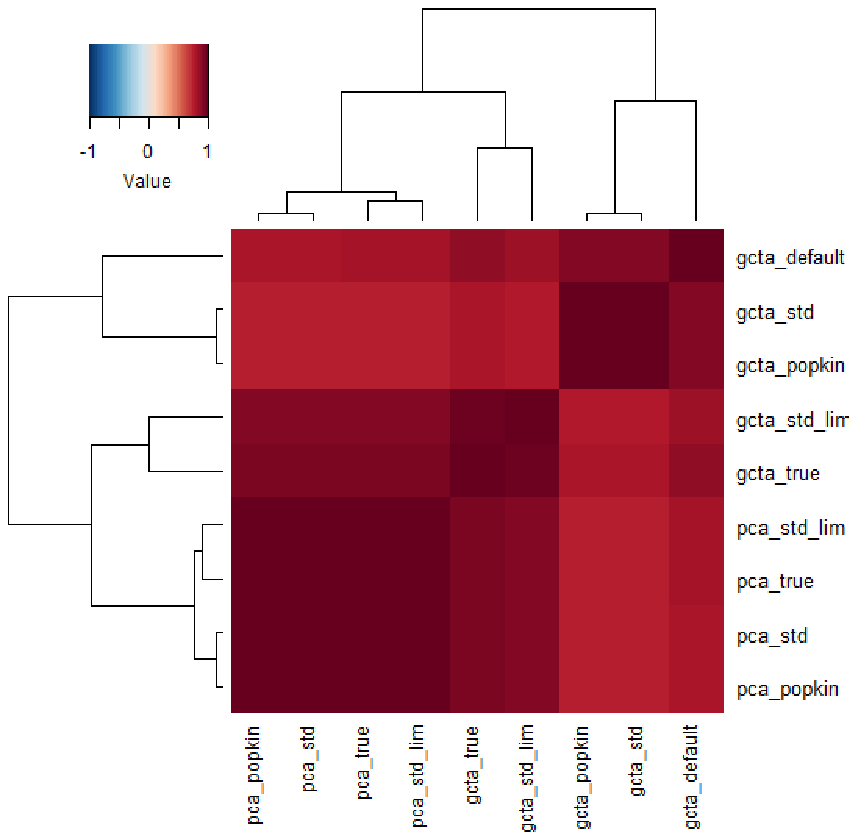
\includegraphics[width=6in]{all_pval.pdf}
  \caption{
    {\bf Heatmap and dendrogram for p-values of GCTA and PCA with different kinship matrices ($m=10,000$).}
  }
  \label{fig:all_pval}
\end{figure}

\begin{figure}[bp!]
  \centering
  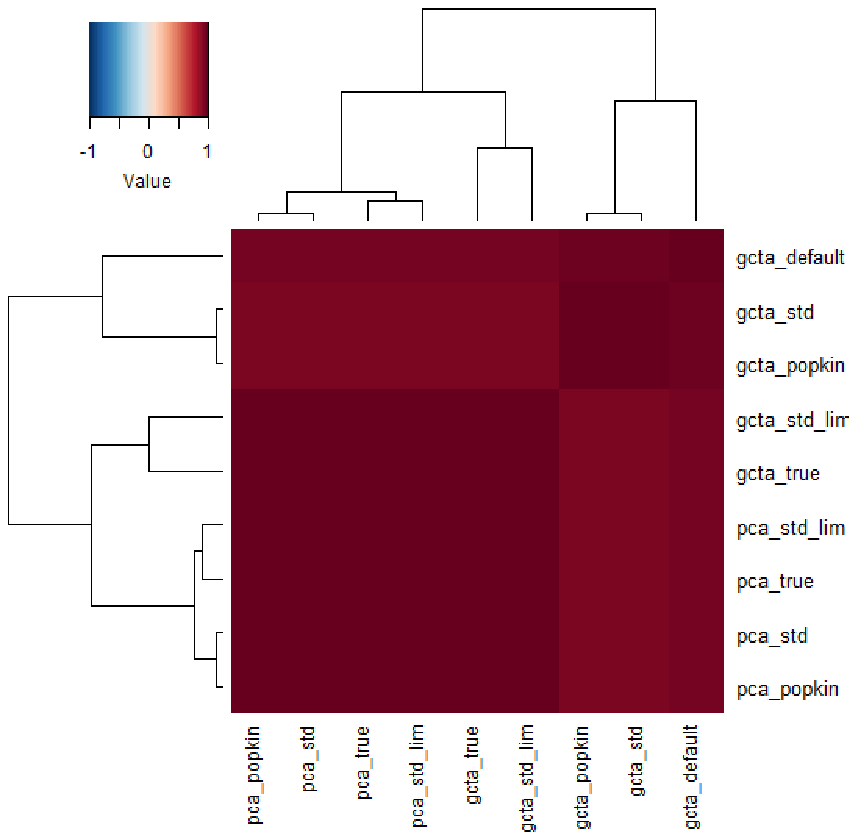
\includegraphics[width=6in]{all_beta_hat.pdf}
  \caption{
    {\bf Heatmap and dendrogram for $\hat{\mathbf{\beta}}$ of GCTA and PCA with different kinship matrices ($m=10,000$).}
  }
  \label{fig:all_beta_hat}
\end{figure}


\subsection{Theoretical justification of empirical observations}

Here, to eliminate random estimation noise from the analysis (which our empirical evaluations suggest play a minor role), we shall focus on the limiting bias of the standard kinship estimator.
Therefore, our theoretical results only consider the true kinship matrix \kinMat and the limit of the standard kinship estimator from \cref{eq:kinship_std}, which can be restated in terms of matrix operations as
$$
\kinMatStdLim
=
\frac{1}{1 - \bar{\varphi}}
\left(
  \kinMat
  + \bar{\varphi} \mathbf{1}_n \mathbf{1}_n^\intercal 
  - \mathbf{\varphi} \mathbf{1}_n^\intercal 
  - \mathbf{1}_n \mathbf{\varphi}^\intercal 
\right)
.
$$
The two kinship matrices are related more succinctly using the centering matrix $\mathbf{C}$:
$$
\kinMatStdLim
=
\frac{1}{1 - \bar{\varphi}}
\mathbf{C} \kinMat \mathbf{C}
, \quad\quad
\mathbf{C}
=
\mathbf{I}_n - \frac{1}{n} \mathbf{1}_n \mathbf{1}_n^\intercal
.
$$

The centering matrix has been well studied, and we review its properties here.
For any length-$n$ vector $\mathbf{v}$ we have
\begin{align*}
  \mathbf{C} \mathbf{v}
  % =
  % \left(\mathbf{I} - \frac{1}{n} \mathbf{1} \mathbf{1}^\intercal\right) \mathbf{v}
  % =
  % \mathbf{I} \mathbf{v} - \frac{1}{n} \mathbf{1} \mathbf{1}^\intercal \mathbf{v}
  =
  \mathbf{v} - \mathbf{1}_n \bar{v}
  ,
\end{align*}
where $\bar{v} = \frac{1}{n} \mathbf{1}_n^\intercal \mathbf{v}$ is the mean value of the elements of $\mathbf{v}$.
Therefore, $\mathbf{v} = \mathbf{1}_n$ gets transformed to the zero vector, so it is an eigenvector with an eigenvalue of zero:
\begin{align*}
  \mathbf{C} \mathbf{1}_n
  % =
  % \mathbf{1} - \mathbf{1}
  =
  \mathbf{0}_n
  .
\end{align*}
Moreover, any vector $\mathbf{v}$ orthogonal to $\mathbf{1}_n$ has a zero mean element ($\bar{v} = 0$) by hypothesis and it is not altered by $\mathbf{C}$ ($\mathbf{C} \mathbf{v} = \mathbf{v}$).
Therefore, the nullspace of $\mathbf{C}$ is spanned by $\mathbf{1}_n$.

This centering matrix provides the key insight as to why PCA and LMM approaches are robust to this specific kinship bias, namely that by fitting the intercept term $\alpha \mathbf{1}_n$ together with the eigenvectors (for PCA) or random effects (in the same rowspace as the eigenvectors; for LMM) of \kinMatStdLim, they complete the rowspace of \kinMatStdLim to equal the rowspace of the true kinship matrix \kinMat plus the intercept.
First we show the following lemma.

\begin{lem}
  $\mathbf{1}_n$ is in the nullspace of \kinMatStdLim but not of \kinMat.
\end{lem}

\begin{proof}
The vector $\mathbf{1}_n$ is not in the nullspace of any true kinship matrix \kinMat, since $\kinMat \mathbf{1}_n \neq \mathbf{0}_n$, which follows since all kinship values are non-negative and the diagonal of the kinship matrix is strictly positive (it has a minimum value of $\frac{1}{2}$).
However, $\mathbf{1}_n$ is in the nullspace of \kinMatStdLim since $\mathbf{C} \mathbf{1}_n = \mathbf{0}_n$:
$$
\kinMatStdLim \mathbf{1}_n
=
\frac{1}{1 - \bar{\varphi}}
\mathbf{C} \kinMat \mathbf{C} \mathbf{1}_n
=
\mathbf{0}_n
.
$$
\end{proof}

Now we may prove the desired theorem.

\begin{thm}
  The rowspace of \kinMat and $\mathbf{1}_n$ equals rowspace of \kinMatStdLim and $\mathbf{1}_n$.
\end{thm}

\begin{proof}
  Since $\mathbf{1}_n$ is in both rowspaces, it suffices to consider vectors $\mathbf{v}$ orthogonal to $\mathbf{1}_n$, which satisfy $\mathbf{C} \mathbf{v} = \mathbf{v}$.
  We shall prove below that any such vector is in the nullspace of \kinMat if and only if it is in the nullspace of \kinMatStdLim.
  Then, since the nullspace of \kinMat and $\mathbf{1}_n$ is the same as the nullspace of \kinMatStdLim and $\mathbf{1}_n$, it follows from the fundamental theorem of linear algebra that their rowspaces are also the same.
  
  If $\mathbf{v}$ is in the nullspace of \kinMat, then $\kinMat \mathbf{v} = \mathbf{0}_n$.
  It follows that
  $$
  \kinMatStdLim \mathbf{v}
  =
  \frac{1}{1 - \bar{\varphi}}
  \mathbf{C} \kinMat \mathbf{C} \mathbf{v}
  =
  \frac{1}{1 - \bar{\varphi}}
  \mathbf{C} \kinMat \mathbf{v}
  =
  \mathbf{0}_n
  ,
  $$
  so $\mathbf{v}$ is also in the nullspace of \kinMatStdLim.
  
  Conversely, if $\mathbf{v}$ is in the nullspace of \kinMatStdLim, then $\kinMatStdLim \mathbf{v} = \mathbf{0}_n$, which implies that
  $
  \mathbf{C} \kinMat \mathbf{C} \mathbf{v}
  =
  \mathbf{C} \kinMat \mathbf{v}
  =
  \mathbf{0}_n
  $.
  Left multiplying by $\mathbf{v}^\intercal$ results in
  $
  \mathbf{v}^\intercal \mathbf{C} \kinMat \mathbf{v}
  =
  \mathbf{v}^\intercal \kinMat \mathbf{v}
  =
  0
  $, which implies that $\mathbf{v}$ is also in the nullspace of the positive-semidefinite matrix \kinMat, as desired.
  If \kinMat were positive definite, then no such $\mathbf{v} \ne \mathbf{0}_n$ would exist (\kinMat would have the trivial nullspace $\{ \mathbf{0}_n \}$).
\end{proof}

\subsubsection{Theoretical justification for PCA genetic association}

In PCA-based genetic association, the desired result follows from the previous theorem, as follows.
Here the goal is to fit the trait $\mathbf{y}$ using a model simiar to our main model in \cref{eq:trait}, namely
\begin{equation}
  \label{eq:pca_gwas}
  \mathbf{y}
  =
  \mathbf{1}_n \alpha + \mathbf{x}_i \beta_i + \mathbf{U}_r \mathbf{\gamma}_r + \mathbf{\epsilon}
  ,
\end{equation}
where instead of including the whole genotype matrix $\mathbf{X}$ as we did in \cref{eq:trait}, here the genotype vector $\mathbf{x}_i$ at a single locus $i$ is fit, and the effect of the rest of the genome is approxiated using the top $r$ eigenvectors of the kinship matrix, contained in the $n \times r$ matrix $\mathbf{U}_r$ and its length-$r$ vector of coefficients $\mathbf{\gamma}_r$.
At each locus $i$ the coefficients $\alpha$, $\beta_i$, and $\mathbf{\gamma}_r$ are fit to minimize the squared error between the observed trait and the model, and the residuals and possibly the degrees of freedom are used to evaluate the significance of the fit for the genotype under the null hypothesis that $\beta_i = 0$.

Here the kinship matrix in question is not the full kinship matrix \kinMat, but its $r$-dimensional approximation $\kinMat_r = \mathbf{U}_r \mathbf{\Lambda}_r \mathbf{U}_r^\intercal$, where $\mathbf{\Lambda}_r$ is an $r \times r$ diagonal matrix of the top $r$ eigenvalues.
One key requirement in need of verification is that $\mathbf{1}_n$ is not in the nullspace of $\kinMat_r$, which certainly holds for reasonable approximations as $\mathbf{1}_n^\intercal \kinMat_r \mathbf{1}_n$ estimates the mean kinship of the data, which is non-zero except for completely unstructured populations.
The other key assumption,
$$
\kinMatStdLim_r \left( 1 - \bar{\varphi} \right)
=
\left( \mathbf{C} \kinMat \mathbf{C} \right)_r
\approx
\mathbf{C} \kinMat_r \mathbf{C},
$$
is only approximately true.
In other words, centering the kinship matrix first and then approximating to the top $r$ dimensions is not exactly equal to first approximating to $r$ dimensions and then centering, although in simulations we found it to be a very good approximation (especially in the absence of family structure, which is where use of PCA is most appropriate anyway [TODO: cite Yao, other papers]).
Therefore, in this case the rowspace of $\kinMat_r$ and $\mathbf{1}_n$ only approximately equals the rowspace of $\kinMatStdLim_r$ and $\mathbf{1}_n$.

The rowspace of $\mathbf{U}_r$ is the same as the rowspace of the $r$-dimensional kinship matrix it is derived from, so either $\kinMat_r$ or $\kinMatStdLim_r$.
Thus, when fitting the model, the space spanned by $\mathbf{1}_n \alpha + \mathbf{U}_r \mathbf{\gamma}_r$ is approximately the same whether the eigenvectors $\mathbf{U}_r$ are derived from the true kinship matrix \kinMat or the limit of the biased estimator \kinMatStdLim, and this is so because the intercept vector $\mathbf{1}_n$ is present in the model.
That implies that, while the coefficients $\alpha$ and $\mathbf{\gamma}_r$ may change when fit based on \kinMat or \kinMatStdLim, the sum of the term $\mathbf{1}_n \alpha + \mathbf{U}_r \mathbf{\gamma}_r$ will be approximately the same, as it is being chosen to minimize the least square error and the subspace is approximately the same, so the value of this solution must be approximately the same.
Thus, the fit of the focal coefficient $\beta_i$ is approximately the same either way, and so is its evaluation of significance (the sum of square errors is also approximately the same).
Therefore, the genetic association test is approximately unchanged when the eigenvectors of either \kinMat or \kinMatStdLim are included as covariates.

\subsubsection{Theoretical justification for LMM genetic association}

...

\section{Discussion}

The biased kinship matrix may be more desireable in PCA, from a numerical standoint, as the resulting eigenvectors are not only orthogonal to each other but also to the intercept (whereas the eigenvectors of the true kinship matrix are not orthogonal to the intercept; see our Lemma).


...

\printbibliography



\end{document}